\chapter{Biophysical background}\label{chap:biophys-back}

\section{Basics of protein structure and their functionality}\label{sec:protein-struct-fun}
Proteins, long polymers of amino acids, constitute the largest fraction (besides water) of a cell. Some proteins have catalytic activity and function as enzymes; others serve as structural elements, signal receptors, or transporters that carry specific substances into or out of cells. Proteins are perhaps the most versatile of all biomolecules; a catalog of their many functions would be very long. The sum of all the proteins functioning in a given cell is the cell’s proteome, and proteomics is the systematic characterization of this protein complement under a specific set of conditions.

Proteins, polynucleotides, and polysaccharides have large numbers of monomeric subunits and thus high molecular weights--in the range of 5,000 to more than 1 million for proteins, up to several billion for nucleic acids, and in the millions for polysaccharides such as starch. Individual lipid molecules are much smaller (Mr 750 to 1,500) and are not classified as macromolecules, but they can associate noncovalently into very large structures. Cellular membranes are built of enormous noncovalent aggregates of lipid and protein molecules. 

Proteins and nucleic acids are linear polymers of simple monomeric subunits; their sequences contain the information that gives each molecule its three-dimensional structure and its biological functions.

All proteins, whether from the most ancient lines of bacteria or from the most complex forms of life, are constructed from the same ubiquitous set of 20 amino acids, covalently linked in characteristic linear sequences. Because each of these amino acids has a side chain with distinctive chemical properties, this group of 20 precursor molecules may be regarded as the alphabet in which the language of protein structure is written. What is most remarkable is that cells can produce proteins with strikingly different properties and activities by joining the same 20 amino acids in many different combinations and sequences. From these building blocks different organisms can make such widely diverse products as enzymes, hormones, antibodies, transporters, muscle fibers, the lens protein of the eye, feathers, spider webs, rhinoceros horn, milk proteins, antibiotics, mushroom poisons, and myriad other substances having distinct biological activities
\cite{nelson2008lehninger}\\
\\
Proteins are one of the essential components of living systems. Along with nucleic acids, polysaccharides, and lipids, proteins constitute the macromolecules that have important roles in biology. 
Nucleic acids, in the form of DNA and RNA, store and distribute the genetic information as needed. Of particular importance is the information that determines the sequences of amino acids that characterize the proteins. Proteins contribute to the structure of an organism and execute most of the tasks required for it to function. Proteins even form part of the complex mechanism by which they are synthesized. Polysaccharides, linear and branched-chain polymers of sugars, provide structural elements, store energy, and when combined with peptides or proteins, play an important role in antigenicity and, more generally, in cellular recognition. Lipids, which include molecules such as fatty acids, phospho- lipids, and cholesterol, serve as energy sources and are the most important components of the membrane structures that organize and compartmentalize cellular function.

In this volume we concentrate on globular proteins, the biological macro- molecules with the greatest functional range. It is for these systems that the relation of function to structure and dynamics is best understood. Most chemical transformations that occur in living systems are catalyzed by en- zymes, the globular proteins that have evolved for executing such specific tasks. As well as enhancing the rates of reactions, sometimes by eight or more orders of magnitude, globular proteins (e.g., repressors) inhibit certain reac- tions (e.g., the transcription of DNA) involved in the mechanism for the con- trol of growth and differentiation. A breakdown of these control mechanisms can lead to unobstructed growth and the development of cancer. Other pro- teins (such as hemoglobin) serve to transport small molecules (such as oxy- gen), electrons, and energy to the appropriate parts of the organism. Anti- body molecules are proteins that protect the organism by specifically recognizing and binding to foreign antigenic substances (such as viruses). Many proteins have structural roles; e.g., fibrous tissue is composed mainly of the protein collagen, and the major functional components of muscle, actin and myosin, are proteins.
Because of this wide range of protein functions and the need to develop specialized proteins for each of them, the number of different proteins in an organism can be very large. The well-studiedbacterium Escherichia coficon- tains about 3000 different kinds of proteins. Since many of them occur in multiple copies, there are a total of about 1 million protein molecules in a single bacterium. In human beings there are estimated to be on the order of lo5to lo6different proteins.

For most globular proteins, the biological function includes an interaction with one or more small molecules (a ligand, hormone, substrate, coenzyme, chromophore, etc.) or another macromolecule. Whether reactive or nonreac- tive systems are being considered, there can be important conformational al- terations in the moleculethat isbound and concomitantchangesin the struc- ture of the macromolecule to which the binding occurs. Such concerted conformationalchangesaretheessentialelementforactivityinsomecases;in others, they play a less significant role. In hormone-receptorbinding, for ex- ample, the structural changes induced in the receptors are fundamental to the transmissionof information. Correspondingly,the conformationaltransi- tion induced by ligand binding in hemoglobin is an integral part of the coop- erative mechanism, Further, in many systems, small motions have been ob- served (e.g., the differences between the ligated and unligated structure of ribonuclease A) that appear to be involved in the function of the protein. Thus any attempt to understand the details of the activity of proteins requires an investigation of the dynamics of the structural fluctuations and their rela- tion to reactivity and conformational change.

In addition to their biological importance, globular proteins are intrinsi- cally interesting systems from the viewpoint of physical chemistry. They are long-chain polymers, but unlike most polymers they have a well-definedaver- age structure. This structure is aperiodic (the “aperiodic crystal” of Schrtid- inger)’ in the sense that it does not have regular repeats. Since the structure is determined by weak, noncovalent, interactions among the elements of the polypeptide chain, large fluctuations are expected. For a complete descrip- tion of proteins, it is important, therefore, to know, in addition to the average structure, the form of the fluctuations that occur, to determine how they take place, and to evaluate their magnitudes and time scales.

Although to chemists and physicists it is self-evident that polymers such as proteins undergo significant fluctuations at room temperature, the classic view of such molecules in their native state had been static in character. This followed from the dominant role of high-resolution X-ray crystallography in providing structural information for these complex systems. The remarkable detail evident in crystal structures led to an image of biomolecules with every atom fixed in place. Tanford suggested that as a result of packing consider- ations “the structure of proteins must be quite rigid.”* D. C. Phillips, who determined the first enzyme crystal structure, has written: “The period 1965- 75 may be described as the decade of the rigid macromolecule. Brass models of DNA and a variety of proteins dominated the scene and much of the think- ing.”3 Molecular dynamics simulations have been instrumental in changing the static view of the structure of biomolecules to a dynamic picture. It is now recognized that the atoms of which biopolymers are composed are in a state of constant motion at ordinary temperatures. The X-ray structure of a protein providesthe average atomic positions, but the atoms exhibit fluidlike motions of sizable amplitudes about these averages. Crystallographers have acceded to this viewpoint and have come so far as sometimes to emphasize the parts of
a molecule they do not see in a crystal structure as evidence of motion or disor- der. The new understanding of protein dynamics subsumes the static picture. Knowledge of the average atomic positions allows discussion of many aspects of biomolecule function in the language of structural chemistry. However, recognition of the importance of fluctuations opens the way for more sophisti- cated and accurate interpretations of protein activity.

Simulations of proteins, as of many other systems (e.g., liquids), can, in principle, provide the ultimate details of motional phenomena. The primary limitation of simulation methods is that they are approximate. It is here that experiment plays an essential role in validating the simulation methods; that is, comparisons with experimental data serve to test the accuracy of the calcu- lated results and provide criteria for improving the methodology. However, the experimental approaches to biomolecular dynamics are limited as to the information that can be obtained from them; e.g., if one is concerned with the time scale of motions, the frequency spectrum covered by experiments such as nuclear magnetic resonance (NMR) is incomplete, so that motional models that are able to rationalize the data can be inaccurate. When experimental comparisons indicate that the simulations are meaningful, their capacity for providing detailed results often makes it possible to examine specific aspects of the atomic motions far more easily than by making measurements. How- ever, at the present stage of development, possible inaccuracies in the simula- tions must be kept in mind in evaluating and applying the results.

\cite{brooks1988proteins}

\subsection{Molecule and macromolecules in biology: the polymeric nature of proteins}\label{ssec:polym-prot}
Proteins, as well the nucleic acids deoxyribonucleic acid (DNA) and ribonucleic acid (RNA), are amongst the most important molecules in biology. 

Generally, molecules are generated by the formation of covalent bonds between pairs of atoms, in which the two atoms share electrons. A covalent bond forms when atoms individually do not have enough electrons for a complete octet: if two atoms can complete their octets by sharing electrons, they can do so by forming a covalent bond. Covalent bonds can be explained only by quantum mechanics, but here it is necessary simply to recognize that covalent bonds are generally not broken in isolation under most conditions experienced in molecular biology. When a covalent bond is broken, as in a chemical or enzymatic reaction, it is generally exchanged with another covalent bond to a different atom. Consequently, covalent bonds define the structures and properties of small molecules, and those of large molecules are determined by the covalent structures of the smaller substituents from which they are made.

Proteins, DNA and RNA are macromolecules characterized by their very large sizes and high molecular weights. These giant molecules can contain many thousands, millions, even billions, of atoms. 
Fortunately, these macromolecules are polymers, i.e. long chains of small molecules built up by the repetition of few relatively simple subunit, the monomers, linked together in a linear fashion to build up the polymeric chains. This polymeric nature of the such biomolecules, in spite of their huge dimension, lead to a simplification of their description -- the basic property of a polymer are determined by those of simpler molecules (its constituent monomers) and by their arrangement within the polymeric chain. These building blocks are four different nucleotides in the case of DNA and RNA, and 20 amino acids in the case of proteins. In each of these cases,  each monomer $i$ of the chain consists of two parts: group $X$ comprises the backbone and is the constant, repeating part of the polymer, while the side-chains (A, B, C, ...) attached to the backbone are variable.

\begin{figure}[h]
\centering
\begin{minipage}[t]{0.8\textwidth}
\centering
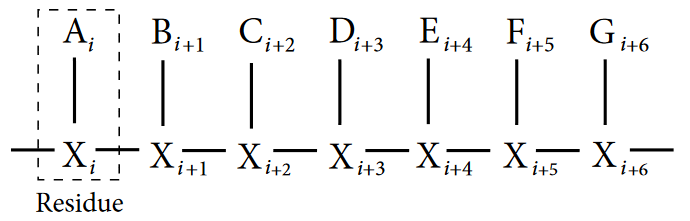
\includegraphics[width=0.7\textwidth]{Polymer.PNG}

\caption{\small{Simple schematization of a short polymer \cite{creighton2010biophysical}.}}

\label{fig:Polymer}
\end{minipage} 
\end{figure}

The backbone of a polymer is the longest series of covalently bonded atoms that create the continuous chain of the molecule. The side-chain is the chemical group of the monomer that is attached to the core part of the molecule in the backbone.

Polymers are subdivided into organic, which have a carbon backbone, and inorganic which have backbones containing only main group elements. In biochemistry, as it is describe in section \ref{ssec:4-lev-prot-struc}, organic backbone chains make up the primary structure of macromolecules.The characteristics and order of the monomer residues in the backbone make a map for the complex structure biological polymers. The backbone is, therefore, directly related to biological molecules' function.

The side-chains connected to the backbone are all the same in homopolymers, as in carbohydrates or polymers made chemically, but they are variable in copolymers; the natural proteins and nucleic acids are extreme examples with several different types. Normally the individual residues are indexed from 1 to $n$, starting from one end of the polymer chain and finishing at the other. The bonds between the residues are numbered similarly, with bond $i$ joining residues $i$ and $i + 1$; there are then $n – 1$ bonds linking the $n$ residues. Normally the backbone primarily has a structural role, while the side-chains contain the functional groups. In spite of the enormous sizes of proteins and nucleic acids, it is possible to determine their detailed covalent structures because, knowing the detailed structures of all the possible monomers, it is necessary only to determine their linear sequence in the polymer.
The detailed structures of the monomers are extremely important, because they determine the global properties of the macromolecule. They occur many times in the polymer, and their structures are multiplied many times over. Many of the monomers occur in only one of several possible isomers; for example natural proteins are composed solely of $l$-amino acids and nucleic acids of $d$-ribose or $d$-deoxyribose. While these details of the structure might seem very minor and mundane, they have extremely important consequences for the three-dimensional (3-D) structures of biopolymers and their functions. These consequences even extend to the macroscopic level; for example, the left/right asymmetry of all but the simplest microorganisms is believed to result from asymmetry at the atomic level of certain molecules.
\cite{creighton2010biophysical}


\subsection{The building blocks of proteins: amino acids}\label{ssec:amino-acids}
Amino acids are organic compounds containing amine (-NH2) and carboxyl (-COOH) functional groups, along with a side chain (R group) specific to each amino acid. The key elements of an amino acid are carbon (C), hydrogen (H), oxygen (O), and nitrogen (N), although other elements are found in the side chains of certain amino acids. About 500 naturally occurring amino acids are known (though only 20 appear in the genetic code) and can be classified in many ways. They can be classified according to the core structural functional groups' locations as alpha- ($\alpha$-), beta- ($\beta$-), gamma- ($\gamma$-) or delta- ($\delta$-) amino acids; other categories relate to polarity, pH level, and side chain group type (aliphatic, acyclic, aromatic, containing hydroxyl or sulfur, etc.). 

In biochemistry, amino acids having both the amine and the carboxylic acid groups attached to the first (alpha-) carbon atom have particular importance. They are known as 2-, $\alpha$-, or $\alpha$-amino acids (generic formula H$_2$NCHRCOOH in most cases\footnote{Proline is an exception to this general formula. It lacks the NH2 group because of the cyclization of the side chain and is known as an imino acid; it falls under the category of special structured amino acids. Note(\url{http://www.chemguide.co.uk/organicprops/aminoacids/background.html}):  For complete accuracy, one of the 20 biologically important amino acids (proline) has a slightly different structure. The ``R'' group is bent into a circle which attaches itself to the nitrogen again in place of one of the hydrogens. This complication doesn't actually make much difference to the chemistry of the compound - the nitrogen still behaves in the same way as it does in the other amino acids.}, where R is an organic substituent known as a ``side chain''); often the term ``amino acid'' is used to refer specifically to these. They include the 22 proteinogenic (``protein-building'') amino acids, which combine into peptide chains (``polypeptides'') to form the building-blocks of a vast array of proteins. These are all L-stereoisomers (``left-handed'' isomers), although a few D-amino acids (``right-handed'') occur in bacterial envelopes, as a neuromodulator (D-serine), and in some antibiotics.

Twenty of the proteinogenic amino acids are encoded directly by triplet codons in the genetic code and are known as ``standard'' amino acids. The other two (``non-standard'' or ``non-canonical'') are selenocysteine (present in many prokaryotes as well as most eukaryotes, but not coded directly by DNA), and pyrrolysine (found only in some archea and one bacterium). Pyrrolysine and selenocysteine are encoded via variant codons; for example, selenocysteine is encoded by stop codon and SECIS element.

\textbf{General structure}\\
In the structure shown at the top of the page, R represents a side chain specific to each amino acid. The carbon atom next to the carboxyl group (which is therefore numbered 2 in the carbon chain starting from that functional group) is called the $\alpha$--carbon. Amino acids containing an amino group bonded directly to the alpha carbon are referred to as alpha amino acids. These include amino acids such as proline which contain secondary amines, which used to be often referred to as ``imino acids''.

\textbf{Proteinogenic amino acids}\\
Amino acids are the structural units (monomers) that make up proteins. They join together to form short polymer chains called peptides or longer chains called either polypeptides or proteins. These polymers are linear and unbranched, with each amino acid within the chain attached to two neighboring amino acids. The process of making proteins encoded by DNA/RNA genetic material is called translation and involves the step-by-step addition of amino acids to a growing protein chain by a ribozyme that is called a ribosome. The order in which the amino acids are added is read through the genetic code from an mRNA template, which is an RNA copy of one of the organism's genes. 

Twenty-two amino acids are naturally incorporated into polypeptides and are called proteinogenic or natural amino acids. Of these, 20 are encoded by the universal genetic code. The remaining 2, selenocysteine and pyrrolysine, are incorporated into proteins by unique synthetic mechanisms. Selenocysteine is incorporated when the mRNA being translated includes a SECIS element, which causes the UGA codon to encode selenocysteine instead of a stop codon. Pyrrolysine is used by some methanogenic archaea in enzymes that they use to produce methane. It is coded for with the codon UAG, which is normally a stop codon in other organisms. This UAG codon is followed by a PYLIS downstream sequence.

\textbf{Physicochemical properties of amino acids}\\
The 20 amino acids encoded directly by the genetic code can be divided into several groups based on their properties. Important factors are charge, hydrophilicity or hydrophobicity, size, and functional groups. These properties are important for protein structure and protein–protein interactions. The water-soluble proteins tend to have their hydrophobic residues (Leu, Ile, Val, Phe, and Trp) buried in the middle of the protein, whereas hydrophilic side chains are exposed to the aqueous solvent. (Note that in biochemistry, a residue refers to a specific monomer within the polymeric chain of a polysaccharide, protein or nucleic acid.) The integral membrane proteins tend to have outer rings of exposed hydrophobic amino acids that anchor them into the lipid bilayer. In the case part-way between these two extremes, some peripheral membrane proteins have a patch of hydrophobic amino acids on their surface that locks onto the membrane. In similar fashion, proteins that have to bind to positively charged molecules have surfaces rich with negatively charged amino acids like glutamate and aspartate, while proteins binding to negatively charged molecules have surfaces rich with positively charged chains like lysine and arginine. There are different hydrophobicity scales of amino acid residues.
Some amino acids have special properties such as cysteine, that can form covalent disulfide bonds to other cysteine residues, proline that forms a cycle to the polypeptide backbone, and glycine that is more flexible than other amino acids. 
Many proteins undergo a range of posttranslational modifications, when additional chemical groups are attached to the amino acids in proteins. Some modifications can produce hydrophobic lipoproteins, or hydrophilic glycoproteins. These type of modification allow the reversible targeting of a protein to a membrane. For example, the addition and removal of the fatty acid palmitic acid to cysteine residues in some signaling proteins causes the proteins to attach and then detach from cell membranes.
\\
WIKIPEDIA

3.1 Amino Acids\\
Amino Acids Proteins are polymers of amino acids, with each amino acid residue joined to its neighbor by a specific type of covalent bond. (The term ``residue'' reflects the loss of the elements of water when one amino acid is joined to another.) Proteins can be broken down (hydrolyzed) to their constituent amino acids by a variety of methods, and the earliest studies of proteins naturally focused on the free amino acids derived from them. Twenty different amino acids are commonly found in proteins. The first to be discovered was asparagine, in 1806. The last of the 20 to be found, threonine, was not identified until 1938. All the amino acids have trivial or common names, in some cases derived from the source from which they were first isolated. Asparagine was first found in asparagus, and glutamate in wheat gluten; tyrosine was first isolated from cheese (its name is derived from the Greek tyros,``cheese''); and glycine (Greek glykos, ``sweet'') was so named because of its sweet taste.

Amino Acids Share Common Structural Features\\
All 20 of the common amino acids are $\alpha$-amino acids. They have a carboxyl group and an amino group bonded to the same carbon atom (the  $\alpha$-carbon) (Fig. 3-2). They differ from each other in their side chains, or R groups, which vary in structure, size, and electric charge, and which influence the solubility of the amino acids in water. In addition to these 20 amino acids there are many less common ones. Some are residues modified after a protein has been synthesized; others are amino acids present in living organisms but not as constituents of proteins. The common amino acids of proteins have been assigned three-letter abbreviations and one-letter symbols (Table 3-1), which are used as shorthand to indicate the composition and sequence of amino acids polymerized in proteins. 

\textbf{Amino Acids Share Common Structural Features}\\
All 20 of the common amino acids are  $\alpha$-amino acids. They have a carboxyl group and an amino group bonded to the same carbon atom (the  $\alpha$ carbon) (Fig. 3-2). They differ from each other in their side chains, or R groups, which vary in structure, size, and electric charge, and which influence the solubility of the amino acids in water. In addition to these 20 amino acids there are many less common ones. Some are residues modified after a protein has been synthesized, others are amino acids present in living organisms but not as constituents of proteins, and two are special cases found in just a few proteins. The common amino acids of proteins have been assigned threeletter abbreviations and one-letter symbols (Table 3-1), which are used as shorthand to indicate the composition and sequence of amino acids polymerized in proteins. 

Two conventions are used to identify the carbons in an amino acid--a practice that can be confusing. The additional carbons in an R group are commonly designated $\beta$, $\gamma$, $\delta$, $\epsilon$, and so forth, proceeding out from the  $\alpha$ carbon. For most other organic molecules, carbon atoms are simply numbered from one end, giving highest priority (C-1) to the carbon with the substituent containing the atom of highest atomic number. Within this latter convention, the carboxyl carbon of an amino acid would be C-1 and the  $\alpha$ carbon would be C-2. In some cases, such as amino acids with heterocyclic R groups, the Greek lettering system is ambiguous and the numbering convention is therefore used.

For all the common amino acids except glycine, the  $\alpha$ carbon is bonded to four different groups: a carboxyl group, an amino group, an R group, and a hydrogen atom (Fig. 3--2; in glycine, the R group is another hydrogen atom). The  $\alpha$-carbon atom is thus a chiral center (p. 17). Because of the tetrahedral arrangement of the bonding orbitals around the  $\alpha$-carbon atom, the four different groups can occupy two unique spatial arrangements, and thus amino acids have two possible stereoisomers. Since they are nonsuperimposable mirror images of each other (Fig. 3--3), the two forms represent a class of stereoisomers called enantiomers

\textbf{Amino Acids Can Be Classified by R Group}\\
Knowledge of the chemical properties of the common amino acids is central to an understanding of biochemistry. The topic can be simplified by grouping the amino acids into five main classes based on the properties of their R groups (Table 3-1), particularly their polarity, or tendency to interact with water at biological pH (near pH 7.0). The polarity of the R groups varies widely, from nonpolar and hydrophobic (water-insoluble) to highly polar and hydrophilic (water-soluble). A few amino acids are somewhat difficult to characterize or do not fit perfectly in any one group, particularly glycine, histidine, and cysteine. Their assignments to particular groupings are the results of considered judgments rather than absolutes.


\textbf{There Are Several Levels of Protein Structure}\\
For large macromolecules such as proteins, the tasks of describing and understanding structure are approached at several levels of complexity, arranged in a kind of conceptual hierarchy. Four levels of protein structure are commonly defined (Fig. 3–16). A description of all covalent bonds (mainly peptide bonds and disulfide bonds) linking amino acid residues in a polypeptide chain is its primary structure. The most important element of primary structure is the sequence of amino acid residues. Secondary structure refers to particularly stable arrangements of amino acid residues giving rise to recurring structural patterns. Tertiary structure describes all aspects of the three-dimensional folding of a polypeptide. When a protein has two or more polypeptide subunits, their arrangement in space is referred to as quaternary structure. Primary structure is the focus of Section 3.4; the higher levels of structure are discussed in Chapter 4.

\textbf{SUMMARY}\\
- Amino acids can be joined covalently through peptide bonds to form peptides and proteins. Cells generally contain thousands of different proteins, each with a different biological activity.\\
- Proteins can be very long polypeptide chains of 100 to several thousand amino acid residues. However, some naturally occurring peptides have only a few amino acid residues. Some proteins are composed of several noncovalently associated polypeptide chains, called subunits. Simple proteins yield only amino acids on hydrolysis; conjugated proteins contain in addition some other component, such as a metal or organic prosthetic group.\\
- The sequence of amino acids in a protein is characteristic of that protein and is called its primary structure. This is one of four generally recognized levels of protein structure.
\cite{nelson2008lehninger}

\subsection{Peptide bonds and polipeptide chains}\label{ssec:peptitde}
\textit{\textbf{POLYPEPTIDE STRUCTURE}}\\
Polypeptide chains make up proteins, which are one of the most important classes of biological
macromolecules, having both structural and catalytic roles. Polypeptide chains are built up during
their biosynthesis from basic building blocks of 21 different amino acids. The amino acids are linked
together in a linear polypeptide chain by forming peptide bonds between them, in an order ordained
by the nucleotide sequence of the corresponding gene for the protein (Section 7.5.F). These 21 amino
acid residues can also be modified post-translationally in very many different ways, to produce even
more variety. The amino acid sequence, appropriately known as the primary structure, identifies a
protein unambiguously, determines all its chemical and biological properties, and specifies (indirectly)
the higher levels of protein structure (Chapters 8 and 9).

7.1. POLYPEPTIDE CHAINS\footnote{A word on nomenclature: a peptide is a shortpolymer of a few amino acid residues with a defined sequence; it usually has properties that are close to those expected from just its constituent amino acids. A polypeptide is a longer chain, with more amino acid residues and a defined sequence; it is usually assumed to remain unfolded and to have no special chemical or physical properties. A polyamino acid has sequences of varying lengths produced by nonspecific random polymerization of one or a few amino acids. A protein is a polypeptide chain with a defined length and amino acid sequence that adopts a specific folded conformation and has special physical and chemical properties.}
Twenty of the amino acids used to synthesize natural proteins have the general structure:

\begin{figure}[h]
\centering
\begin{minipage}[t]{0.325\textwidth}
\centering
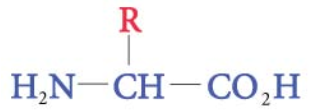
\includegraphics[width=\textwidth]{GenericAminoAcids.PNG}


\label{fig:GenericAminoAcids}
\end{minipage} 
\end{figure}

they differ only in the chemical structures of the side-chain, R. The amino group and the carboxyl
group give this class of compounds its name. At physiological pH values, both groups are ionized,
and this zwitterion is the common form of the amino acid in solution. The exceptional amino acid,
proline, differs in that its side-chain is bonded to the N atom of the amino group, which is then a
secondary amine, and proline is an imino acid:
The central C" atom is asymmetric in 20 of the amino acids and is always the L-isomer:
The L-isomer can be readily identified by looking down from the H atom to the C atom and
remembering the "CORN rule": the other groups should occur in the clockwise sequence CO, R
(side-chain) and N. Glycine is the exception, in that its side-chain is simply another H atom, so the
C" atom is not chiral.
Amino acids are linked together by peptide bonds formed by condensation of the a-carboxyl group
of one amino acid with the a-amino group of another, producing a dipeptide (Figure \ref{fig:PeptideFormation}). Repeated
condensation of additional amino acids produces tripeptides, tetrapeptides, and so on.

\begin{figure}[h]
\centering
\begin{minipage}[t]{0.8\textwidth}
\centering
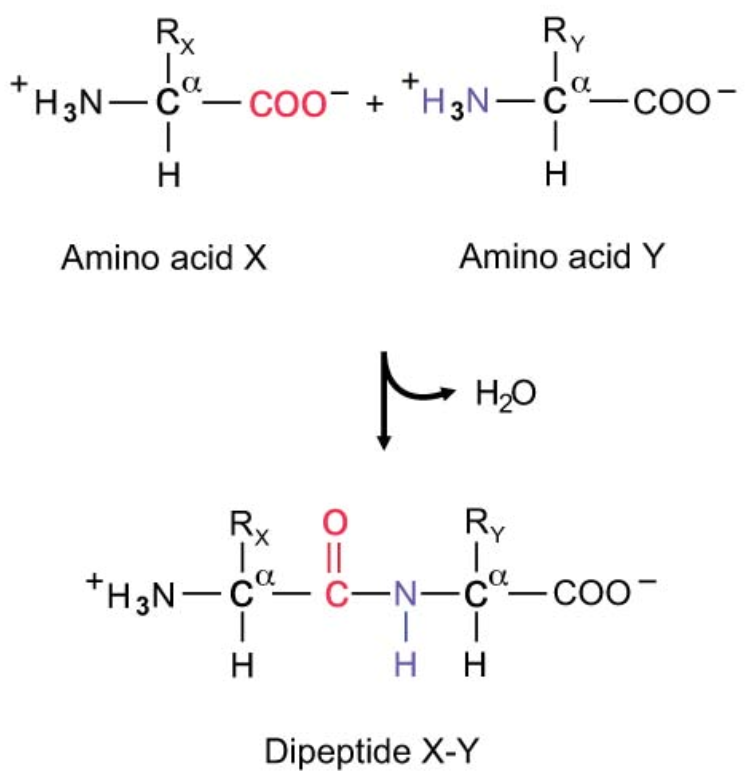
\includegraphics[width=0.6\textwidth]{PeptideFormation.PNG}

\caption{\small{General scheme for formation of a dipeptide XY from two amino acids, X and Y, by reaction of the carboxyl group of amino acid X with the amino group of amino acid Y. The R group attached to Ca is variable depending on the type of amino acid: R, and R,\cite{creighton2010biophysical}.}}

\label{fig:PeptideFormation}
\end{minipage} 
\end{figure}


POLYPEPTIDE CONFORMATION
The structures of all molecules extend to three dimensions. Two-dimensional (2-D) chemical
representations usually suffice for small molecules because their three-dimensional (3-D) structures
are defined reasonably well by the fixed bond lengths and bond angles of their covalent structures.
These representations are not sufficient for larger molecules, however, because rotations about
the many covalent bonds dramatically alter the relative positions of all the atoms. 3-D aspects of
structure are especially important for polymers such as nucleic acids and proteins, in which many
bonds can rotate. Polymers have an intrinsic tendency to be very flexible, when no one structure,
or conformation (Section 1.2), is sufficiently more stable than all the others to predominate, but
nevertheless many biological macromolecules, especially the proteins and nucleic acids (Chapters 2,
4 and 9), tend to adopt single, stable conformations.
The abilities of polypeptide chains to adopt a wide variety of 3-D conformations is crucial so that they
can carry out their many different functions (Chapters 12–15). These conformational properties of
polypeptide chains are controlled to a great extent by the flexibility of the polypeptide backbone and
by local interactions with amino acid side-chains, which are described in this chapter.

8.2. RANDOM-COIL POLYPEPTIDE CHAINS
The substantial flexibility of the polypeptide chain gives it significant conformational entropy (Section
1.3) and makes the random coil the most favored conformation under many conditions. Most studies
of random polypeptide chains have been done with polyamino acids, in which one type of amino acid
is polymerized into a homopolypeptide chain. Yet it is not clear that any polypeptide chain adopts
a completely random-coil conformation, as various interactions can usually be observed, especially
between chemical groups close in the covalent structure. Many unfolded proteins that previously were
thought to approximate random coils are now thought to contain significant amounts of nonrandom
conformation, like that observed in poly(Pro) II (Section 8.3.D), but this might just be the most
favorable stereochemistry for the polypeptide chain.
\cite{creighton2010biophysical}

\subsection{Four levels of protein structure}\label{ssec:4-lev-prot-struc}

\textbf{The Structure of Proteins: Primary Structure} \\
What is it that makes one protein an enzyme, another a hormone, another a structural protein, and still another an antibody? How do they differ chemically? The most obvious distinctions are structural, and to protein structure we now turn.
The structure of large molecules such as proteins can be described at several levels of complexity, arranged in a kind of conceptual hierarchy. Four levels of protein structure are commonly defined (Fig. 3-23). A description of all covalent bonds (mainly peptide bonds and disulfide bonds) linking amino acid residues in a polypeptide chain is its primary structure. The most important element of primary structure is the sequence of amino acid residues. Secondary structure refers to particularly stable arrangements of amino acid residues giving rise to recurring structural patterns. Tertiary structure describes all aspects of the three-dimensional folding of a polypeptide. When a protein has two or more polypeptide subunits, their arrangement in space is referred to as quaternary structure. 

Differences in primary structure can be especially informative. Each protein has a distinctive number and sequence of amino acid residues. The primary structure of a protein determines how it folds up into its unique three-dimensional structure, and this in turn determines the function of the protein.

\textbf{The Function of a Protein Depends on Its Amino Acid Sequence}\\
The bacterium Escherichia coli produces more than 3,000 different proteins; a human has $\sim$20,000 genes encoding a much larger number of proteins (through genetic processes discussed in Part III of this text). In both cases, each type of protein has a unique amino acid sequence that confers a particular three-dimensional structure. This structure in turn confers a unique function. Some simple observations illustrate the importance of primary structure, or the amino acid sequence of a protein. First, as we have already noted, proteins with different functions always have different amino acid sequences. Second, thousands of human genetic diseases have been traced to the production of defective proteins. The defect can range from a single change in the amino acid sequence (as in sickle cell disease, described in Chapter 5) to deletion of a larger portion of the polypeptide chain (as in most cases of Duchenne muscular dystrophy: a large deletion in the gene encoding the protein dystrophin leads to production of a shortened, inactive protein). 
Finally, on comparing functionally similar proteins from different species, we find that these proteins often have similar amino acid sequences.
Thus, a close link between protein primary structure and function is evident. Is the amino acid sequence absolutely fixed, or invariant, for a particular protein? No; some flexibility is possible. An estimated 20\% to 30\% of the proteins in humans are polymorphic, having amino acid sequence variants in the human population. Many of these variations in sequence have little or no effect on the function of the protein. Furthermore, proteins that carry out a broadly similar function in distantly related species can differ greatly in overall size and amino acid sequence. Although the amino acid sequence in some regions of the primary structure might vary considerably without affecting biological function, most proteins contain crucial regions that are essential to their function and thus have sequences that are conserved. The fraction of the overall sequence that is critical varies from protein to protein, complicating the task of relating sequence to three-dimensional structure, and structure to function. 

OLD VERSION\\
the important relationship between amino acid sequence and biological function. First, as we have already noted, proteins with different functions always have different amino acid sequences. Second, thousands of human genetic diseases have been traced to the production of defective proteins. Perhaps one-third of these proteins are defective because of a single change in their amino acid sequence; hence, if the primary structure is altered, the function of the protein may also be changed. Finally, on comparing functionally similar proteins from different species, we find that these proteins often have similar amino acid sequences. An extreme case is ubiquitin, a 76-residue protein involved in regulating the degradation of other proteins. The amino acid sequence of ubiquitin is identical in species as disparate as fruit flies and humans. Is the amino acid sequence absolutely fixed, or invariant, for a particular protein? No; some flexibility is possible. An estimated 20\% to 30\% of the proteins in humans are polymorphic, having amino acid sequence variants in the human population. Many of these variations in sequence have little or no effect on the function of the protein. Furthermore, proteins that carry out a broadly similar function in distantly related species can differ greatly in overall size and amino acid sequence. Although the amino acid sequence in some regions of the primary structure might vary considerably without affecting biological function, most proteins contain crucial regions that are essential to their function and whose sequence is therefore conserved. The fraction of the overall sequence that is critical varies from protein to protein, complicating the task of relating sequence to three-dimensional structure, and structure to function. 

\textbf{Amino Acid Sequences Provide Important Biochemical Information}\\
Knowledge of the sequence of amino acids in a protein can offer insights into its three-dimensional structure and its function, cellular location, and evolution. Most of these insights are derived by searching for similarities between a protein of interest and previously studied proteins. Thousands of sequences are known and available in databases accessible through the Internet. A comparison of a newly obtained sequence with this large bank of stored sequences often reveals relationships both surprising and enlightening. Exactly how the amino acid sequence determines three-dimensional structure is not understood in detail, nor can we always predict function from sequence. However, protein families that have some shared structural or functional features can be readily identified on the basis of amino acid sequence similarities. Individual proteins are assigned to families based on the degree of similarity in amino acid sequence. Members of a family are usually identical across 25\% or more of their sequences, and proteins in these families generally share at least some structural and functional characteristics. Some families, however, are defined by identities involving only a few amino acid residues that are critical to a certain function. A number of similar substructures, or “domains” (to be defined more fully in Chapter 4), occur in many functionally unrelated proteins. These domains often fold into structural configurations that have an unusual degree of stability or that are specialized for a certain environment. Evolutionary relationships can also be inferred from the structural and functional similarities within protein families. Certain amino acid sequences serve as signals that determine the cellular location, chemical modification, and half-life of a protein. Special signal sequences, usually at the amino terminus, are used to target certain proteins for export from the cell; other proteins are targeted for distribution to the nucleus, the cell surface, the cytosol, or other cellular locations. Other sequences act as attachment sites for prosthetic groups, such as sugar groups in glycoproteins and lipids in lipoproteins. Some of these signals are well characterized and are easily recognized in the sequence of a newly characterized protein (Chapter 27). 

\textbf{SUMMARY 3.4 The Structure of Proteins: Primary Structure}\\
\begin{itemize}
\item Differences in protein function result from differences in amino acid composition and sequence. Some variations in sequence may occur in a particular protein, with little or no effect on its function.
\item Protein sequences are a rich source of information about protein structure and function, as well as the evolution of life on Earth. Sophisticated methods are being developed to trace evolution by analyzing the slow changes in amino acid sequences of homologous proteins.
\end{itemize}

\textbf{The ThreeDimensional Structure of Proteins}\\
The covalent backbone of a typical protein contains hundreds of individual bonds. Because free rotation is possible around many of these bonds, the protein can assume an unlimited number of conformations. However, each protein has a specific chemical or structural function, strongly suggesting that each has a unique three-dimensional structure (Fig. 4–1). By the late 1920s, several proteins had been crystallized, including hemoglobin (Mr 64,500) and the enzyme urease (Mr 483,000). Given that the ordered array of molecules in a crystal can generally form only if the molecular units are identical, the simple fact that many proteins can be crystallized provides strong evidence that even very large proteins are discrete chemical entities with unique structures. This conclusion revolutionized thinking about proteins and their functions.

 First, the three-dimensional structure or structures taken up by a protein are determined by its amino acid sequence. Second, the function of a typical protein depends on its structure. Third, most isolated proteins exist in one or a small number of stable structural forms. Fourth, the most important forces stabilizing the specific structures maintained by a given protein are noncovalent; the hydrophobic effect is particularly important. Fifth, amid the huge number of unique protein structures, we can recognize some common structural patterns that help to organize our understanding of protein architecture. Finally, protein structures are not static. All proteins undergo changes in conformation ranging from subtle to dramatic. Parts of many proteins have no discernible structure. For some proteins or parts of proteins, a lack of definable structure is critical to their function.

OLD VERSION\\
First, the three-dimensional structure of a protein is determined by its amino acid sequence. Second, the function of a protein depends on its structure. Third, an isolated protein usually exists in one or a small number of stable structural forms. Fourth, the most important forces stabilizing the specific structures maintained by a given protein are noncovalent interactions. Finally, amid the huge number of unique protein structures, we can recognize some common structural patterns that help us organize our understanding of protein architecture.
These themes should not be taken to imply that proteins have static, unchanging three-dimensional structures. Protein function often entails an interconversion between two or more structural forms. The dynamic aspects of protein structure will be explored in Chapters 5 and 6.
The relationship between the amino acid sequence of a protein and its three-dimensional structure is an intricate puzzle that is gradually yielding to techniques used in modern biochemistry. An understanding of structure, in turn, is essential to the discussion of function in succeeding chapters. We can find and understand the patterns within the biochemical labyrinth of protein structure by applying fundamental principles of chemistry and physics.

\textbf{Overview of Protein Structure}\\
The spatial arrangement of atoms in a protein or any part of a protein is called its conformation. The possible conformations of a protein or protein segment include any structural state it can achieve without breaking covalent bonds. A change in conformation could occur, for example, by rotation about single bonds. Of the many conformations that are theoretically possible in a protein containing hundreds of single bonds, one or (more commonly) a few generally predominate under biological conditions. The need for multiple stable conformations reflects the changes that must take place in most proteins as they bind to other molecules or catalyze reactions. The conformations existing under a given set of conditions are usually the ones that are thermodynamically the most stable—that is, having the lowest Gibbs free energy (G). Proteins in any of their functional, folded conformations are called native proteins. For the vast majority of proteins, a particular structure or small set of structures is critical to function. However, in many cases, parts of proteins lack discernible structure. These protein segments are intrinsically disordered. In a few cases, entire proteins are intrinsically disordered, yet are fully functional. 

\textbf{Protein Function}\\
Knowing the threedimensional structure of a protein is an important part of understanding protein function, and modern structural biology often includes insights into molecular interactions. However, the protein structures we have examined so far are deceptively static. Proteins are dynamic molecules. Their interactions are affected in physiologically important ways by sometimes subtle, sometimes striking changes in protein conformation. In this chapter and the next, we explore how proteins interact with other molecules and how their interactions are related to dynamic protein structure. 
We divide these interactions into two types. In some interactions, the result is a reaction that alters the chemical configuration or composition of the interacting molecule, with the protein acting as a reaction catalyst, or enzyme; we discuss enzymes and their reactions in Chapter 6. In other interactions, neither the chemical configuration nor the composition of the interacting molecule is changed, and such interactions are the subject of this chapter.
It may seem counterintuitive that a protein’s interaction with another molecule could be important if it does not alter the associated molecule. Yet, transient interactions of this type are at the heart of complex physiological processes such as oxygen transport, immune function, and muscle contraction --all topics we examine here. The proteins that carry out these processes illustrate several key principles of protein function, some of which will be familiar from Chapter 4: 
The functions of many proteins involve the reversible binding of other molecules. A molecule bound reversibly by a protein is called a ligand. A ligand may be any kind of molecule, including another protein. The transient nature of protein-ligand interactions is critical to life, allowing an organism to respond rapidly and reversibly to changing environmental and metabolic circumstances. A ligand binds at a site on the protein called the binding site, which is complementary to the ligand in size, shape, charge, and hydrophobic or hydrophilic character. Furthermore, the interaction is specific: the protein can discriminate among the thousands of different molecules in its environment and selectively bind only one or a few types. A given protein may have separate binding sites for several different ligands. These specific molecular interactions are crucial in maintaining the high degree of order in a living system. (This discussion excludes the binding of water, which may interact weakly and nonspecifically with many parts of a protein. In Chapter 6, we consider water as a specific ligand for many enzymes.) Proteins are flexible. Changes in conformation may be subtle, reflecting molecular vibrations and small movements of amino acid residues throughout the protein. A protein flexing in this way is sometimes said to “breathe.” Changes in conformation may also be more dramatic, with major segments of the protein structure moving as much as several nanometers. Specific conformational changes are frequently essential to a protein’s function. The binding of a protein and ligand is often coupled to a conformational change in the protein that makes the binding site more complementary to the ligand, permitting tighter binding. The structural adaptation that occurs between protein and ligand is called induced fit. In a multisubunit protein, a conformational change in one subunit often affects the conformation of other subunits. Interactions between ligands and proteins may be regulated, usually through specific interactions with one or more additional ligands. These other ligands may cause conformational changes in the protein that affect the binding of the first ligand. 

The enzymes represent a special case of protein function. They bind and chemically transform other molecules. The molecules acted upon by enzymes are called reaction substrates rather than ligands, and the ligand-binding site is called the catalytic site or active site. As you will see, the themes in our discussion of noncatalytic functions of proteins in this chapter--binding, specificity, and conformational change--are continued in Chapter 6, with the added element of proteins participating in chemical transformations.
\cite{nelson2008lehninger}
\\
PROTEIN STRUCTURE\\
Most dynamic activities in cells and organisms are caused by proteins, and the key to understanding
these phenomena is their structures. Protein structures, however, consist of many atoms, often
thousands, and can be extremely complex. Natural proteins are also folded into precise threedimensional
(3-D) structures and are very different from random-coil forms of the polypeptide chain
(Section 8.2), in that most of their covalent bonds adopt a single dihedral angle (Section 1.2.B) and
Cys residues pair in specific disulfide bonds (Section 7.2.1.5), rather than the spectrum possible with
disordered polypeptide chains (Table 7-3); this generally results in a folded conformation that can be
considered unique. It is also very compact. No changes in covalent structure need occur when these
folded conformations are adopted, except for the disulfide bonds that might be formed between Cys
residues (Section 7.2.1.5); therefore the folded structure represents just one conformation of the many
that are possible with a disordered polypeptide chain. With 20 different amino acid residues having
diverse physical and chemical properties, a huge variety of protein sequences and conformations are
possible. Some proteins are globular and water-soluble, others exist buried within membranes, while
others adopt elongated and extended structures that serve primarily structural roles (Section 8.5).
Protein structure is most impressive in its diversity.
Each protein is identified uniquely by its amino acid sequence, which is determined by the
sequence of the gene from which the protein is produced, using the genetic code (Section 7.5.F). The
amino acid sequence determines all further aspects of the structure of the protein and, consequently,
its functions. It has become customary to dissect protein structure into four levels (Figure 9-1).
The primary structure is the amino acid sequence. The secondary structure is any regular local
structure of a linear segment of polypeptide chain, such as a helix or an extended strand (Section
8.3). The tertiary structure is the overall topology of the folded polypeptide chain. The quaternary
structure is the aggregation of the individual polypeptides by specific interactions between them.
As more protein structures have been determined, two intermediate levels of structure have become
apparent; one comprises several elements of secondary structure packed together and is known as the
supersecondary structure or motif; the other is the domain, which can be one self-contained part
of a tertiary structure.
Details of virtually all the known structures of proteins can be obtained from the Protein Data Bank
(PDB; www.rcsb.org). They can be viewed most readily online using the program Jmol at http://
firstglance.jmol.org.

\begin{figure}[h]
\centering
\begin{minipage}[t]{0.875\textwidth}
\centering
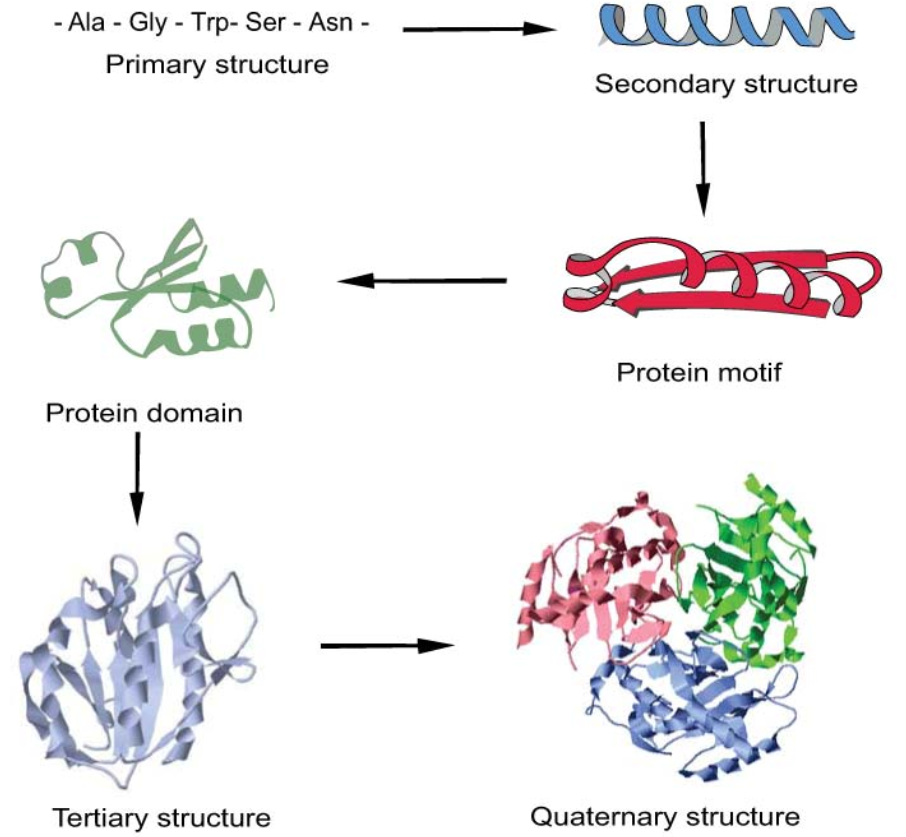
\includegraphics[width=0.9\textwidth]{ProteinStructure.PNG}

\caption{\small{Different levels of  protein structure, from primary to quaternary. Helices are depicted as coils and P-strands as arrows. The primary structure is the amino acid sequence of the polypeptide chain. The secondary structure example shown is an a-helix; the protein motif is  a pap motif, where P is a P-strand, a an a-helix and the motif produces a parallel P-sheet. The protein domain is a folded structure that is stable in isolation. The tertiary structure is the folded structure of a complete polypeptide chain, in this case that of flavodoxin. The quaternary structure is produced by the aggregation of multiple polypeptide chains; in this case it is the homotrimer of  chloramphenicol acetyltransferase. 
\cite{creighton2010biophysical}.}}

\label{fig:ubq}
\end{minipage} 
\end{figure}

\begin{figure}[h]
\centering
\begin{minipage}[t]{0.6\textwidth}
\centering
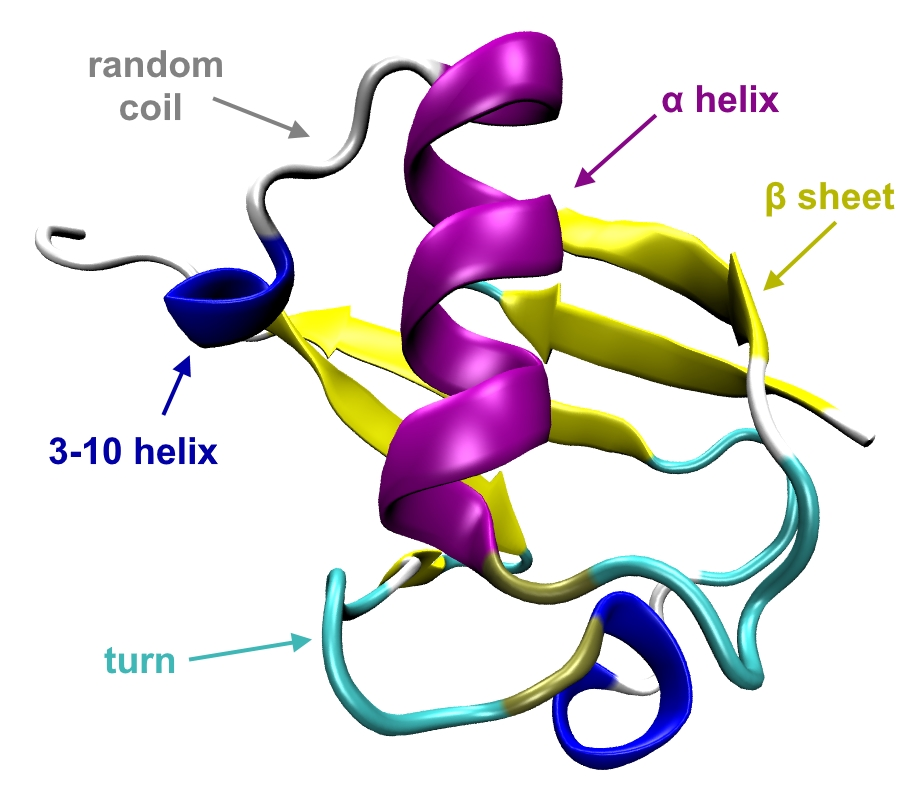
\includegraphics[width=\textwidth]{ubq-label.jpg}

\caption{\small{}}

\label{fig:ProteinStructure}
\end{minipage} 
\end{figure}

\subsection{Protein functions}\label{ssec:prot-fun}

\section{Basics of protein structure and their functionality}
\subsection{Protein as Macromolecules}


\subsection{Protein structure}






TIZIO\\


\section{Basics of protein structure and their functionality}



\section{Protein-ligand binding}
%\section{Ligand binding process}
The biological functions of macromolecules almost invariably depend upon their direct physical
interaction with other molecules. All organisms and cells survive only because they interact
effectively with their environments. Extraneous molecules must be distinguished as either useful or
dangerous and dealt with accordingly. Organisms have sophisticated sensory organs for being aware
of their environments. At a lower level, all cells have a variety of receptors for different molecules
for this purpose. Virtually every small molecule in a cell was first bound specifically by the enzyme
that produced it or by the receptor on the cell that enabled it to enter that cell. Every aspect of the
structure, growth and replication of an organism depends upon proteins binding small molecules,
other proteins, nucleic acids, polysaccharides or lipids. Of crucial importance is the specificity of such
interactions. In the crowded interior of a cell, each molecule must interact only with the appropriate
molecules and not with any of the others that are present, often in extremely high concentrations.
The following discussion will be general but will apply primarily to proteins binding smaller ligands,
such as their substrates for enzymatic reactions, although the catalytic events that take place after
binding on the enzyme will be saved for Chapter 14. The interactions between nucleic acids and
proteins are described in Chapter 13; base-pairing interactions between complementary strands of
DNA and RNA are described in Chapter 5, and their interactions with small molecules are described
in Sections 2.5 and 14.6.
Only binding to specific sites on a protein will be considered here, and phenomena such as the
electrostatic binding of counterions to a polyanion or polycation (Section 2.3) will not be considered
here as ligand binding. Likewise, little attention will be given to interactions with normal components
of the solvent, such as water molecules and co-solvents in the case of water-soluble proteins and lipids
in the case of membrane proteins. These interactions are not fundamentally different but they do
not occur at specific sites on the protein and are generally weak, occurring only because the solvent
molecules are present at high concentrations

12.1. GENERAL PROPERTIES OF PROTEIN-LIGAND INTERACTIONS
Proteins usually bind only very specific ligands and can discriminate between closely related
molecules. This specificity is usually crucial for their biological functions. Proteins are generally
classified according to the purpose and consequences of their binding; examples are structural
proteins, enzymes, repressors, lectins, toxins, immunoglobulins, hormones, receptors, membrane
transport proteins and proteins of motility. The physical principles of the interactions are similar in
all these cases. The following discussion focuses on the protein; whatever molecule it interacts with,
even if another protein, is designated the ligand. A protein with its ligand bound is known as the holo
form; that without the ligand is the apo form. Some examples of specific complexes are illustrated in
Figure 12- 1.
\cite{creighton2010biophysical}

\section{The free-energy landscape and conformational entropy}
%\section{Hydration water}

The understanding of how ligands bind to proteins is of fundamental importance in biology and medicine.\footnote{The structures of protein-ligand complexes at atomic resolution make possible, for example, the design of small-molecule drugs for the treatment of disease \cite{dunn2001protein}.} Indeed, the protein-ligand interactions are crucial for the determination of the biological functions and, as a consequence, these interactions underlie almost all processes occuring in living organisms. In fact, every aspect of the structure, growth and replication of an organism depends in general on the way the proteins bind ligands (i.e. small molecules, nucleic acids, peptides, other proteins, polysaccharides or lipid) \cite{creighton2010biophysical}.

The association processes that bring to the formation of the binding between a protein and its ligand, also known as \textcolor{ForestGreen}{protein-ligand} complexation\footnote{A protein–ligand complex is a complex of a protein bound with a ligand.}, occurs when the free-energy of the whole system (protein, ligand and solvent) is lower for the complexed state, $G^\text{(c)}$, than for uncomplexed one, $G^\text{(uc)}$. Defining the difference between $G^\text{(c)}$ and $G^\text{(uc)}$ as $\Delta G$, it is possible to divide $\Delta G$ into the following two terms:
\begin{equation*}
\label{free-en}
\Delta G = G^\text{(c)} - G^\text{(uc)} = \Delta H - T \Delta S
\end{equation*}
where $\Delta H$ is the change in enthalpy due to the electrostatic interactions, while $\Delta S$ is the change in entropy due to the variation of the number of microscopic configurations for the whole system that corresponds to the new macroscopic state, namely, the solvated protein-ligand complex.
%\begin{align*}
%\label{c-uc}
%&\Delta G < 0 \quad \Longrightarrow \quad \text{\textit{the complex state is stable}} \\
%&\Delta G > 0 \quad \Longrightarrow \quad \text{\textit{the uncomplex state is stable}}
%\end{align*}

Water deeply buried in proteins is considered to be an integral part of the folded structure. Such structural water molecules make strong H bonds with polar groups of the surrounding protein and therefore are believed totightentheproteinmatrix.

Studying this association processes, it is useful to identify the favorable and unfavorable contributions to the change in the free-energy of the system. Most of the unfavorable contribution is due to the loss of the three translational and three rotational degrees of freedom that lead to a considerable decrease of the entropy of the system. Generally, it is assumed that this contribution is offset by favorable enthalpy of binding and entropic contributions, such as the hydrophobic effect, changes in the protonation state and solvent or counterion release\footnote{The solvent entropy change arising mainly from surface burial that results in solvent release upon binding, often makes a favorable contribution to the binding entropy due to its large positive value. A counterion (pronounced as two words, i.e. ``counter'' + ``ion'', and sometimes written as two words) is the ion that accompanies an ionic species in order to maintain electric neutrality. In table salt (NaCl), the sodium cation is the counterion for the chlorine anion and vice versa. For most protein-nucleic acid complexes, for example, a major contributions to the binding free energy associated with formation of the complexes is the increase in entropy due to counterion release from the nucleic acid that results from electrostatic interactions \cite{mascotti1990thermodynamic}. On the other hand,}. Nevertheless, there are other mechanisms, due to the creation or suppression of new internal degrees of freedom in the complex, that induce a change of the intrinsic entropy of the association by which a significant amount of entropy can be lost or recovered \cite{tidor1994contribution}. For this reason, it useful to divide $\Delta S$ in two contributions:
\begin{equation*}
\label{entropy-variation:total}
\Delta S = \Delta S_\text{intr} + \Delta S_\text{solv}
\end{equation*}
where $\Delta S_\text{solv}$ is the entropy change arising from accompanying modifications of interactions with the solvent, while $\Delta S_\text{intr}$ is the intrinsic change of the entropy involved in creating a dimer from two separate molecules \cite{steinberg1963entropy}. In particular, $\Delta S_\text{intr}$ represents the variation of the entropy due to the change of the number of configurations for the protein-ligand system upon the complexation (without considering the solvent) and, because of that, $\Delta S_\text{intr}$ is usually known as $\Delta S_\text{config} = S_\text{config}^\text{(c)} - S_\text{config}^\text{(uc)}$, where $S_\text{config}^\text{(c)}$ and $S_\text{config}^\text{(uc)}$ are the configuration entropy of the complexed and uncomplexed state, respectively. 

For each of these states, the configurational entropy represents a measure of the extent of the configuration space accessible to the internal degrees of freedom of the protein-ligand subsystem. In this way, the concept of configurational entropy is strongly connected to that of free-energy landscape and, as a consequece, a full characterization of the protein-ligand free-energy landscape is of fundamental importance to understand the relationship between the configurational entropy and the protein structure and the variation of these quantities upon ligand binding and conformational change. Unfortunately, the configurational entropy is known as one of the most difficult thermodynamic quantities to estimate and the characterization of the protein free-energy landscape is a difficult task due to its complexity and, in particular, to the fact that it is rugged, i.e., it comprises numerous local minima separated by low free-energy barriers \cite{chong2015dissecting}. 

In this regard, it was a keen insight to suppose that the protein configurational entropy $S_\text{config}$ may be characterized just by two terms, namely: 
\begin{equation*}
\label{entropy-variation:configurational}
\Delta S_\text{intr} \equiv \Delta S_\text{config} = \Delta S_\text{conf} + \Delta S_\text{vib}
\end{equation*}
where  $S_\text{conf}$ is the conformational components of the configurational entropy associated with the number of accessible free-energy wells \footnote{Sometimes, specially studying the protein folding phenomena, $\Delta S_\text{config}$ and  $\Delta S_\text{conf}$ might be used interchangeably even if they are not the same. This is why, in the protein folding process usually $\Delta S_\text{vib} \simeq 0$, hence $\Delta S_\text{conf} \simeq S_\text{conf}$ \cite{karplus1987configurational}.}, whereas $S_\text{vib}$ is the vibrational component that reflects the average width of the individual wells \cite{chong2015dissecting, karplus1987configurational}.%\footnote{Although attempts to dissect the relative magnitudes of different thermodynamic effects have been criticized as not formally correct, it remains helpful in understanding protein stability to estimate these individual contributions 
%\cite{doig1995side}.}.

\begin{figure}[h]
\centering
\begin{minipage}[t]{0.8\textwidth}
\centering
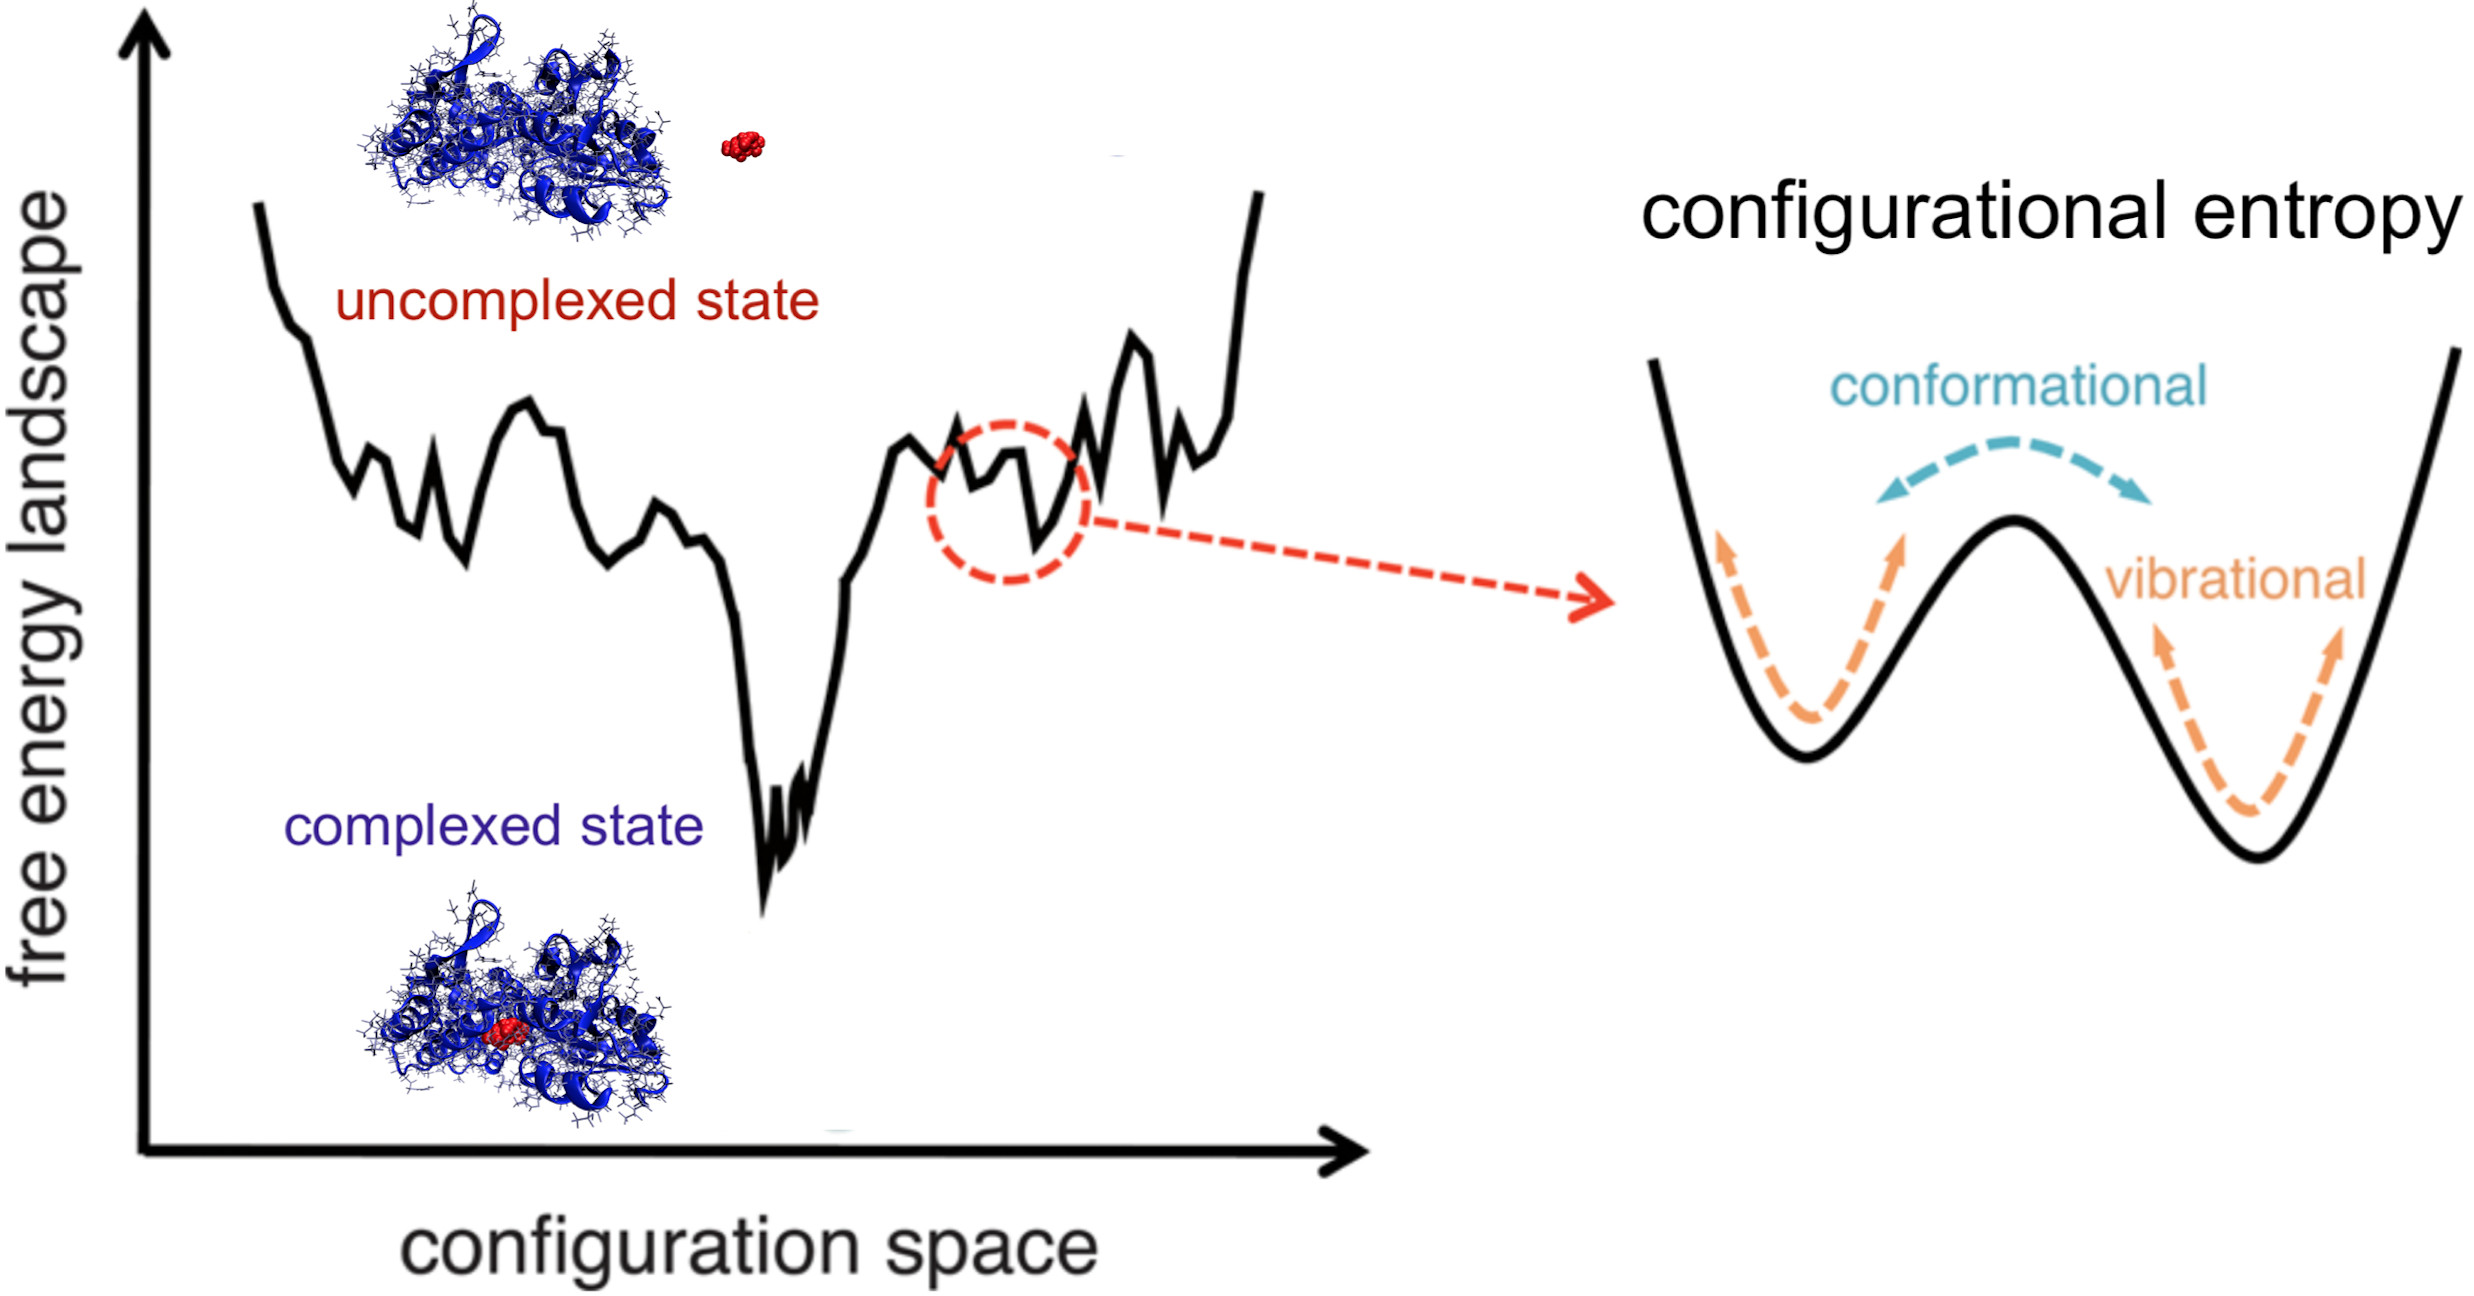
\includegraphics[width=0.93\textwidth]{free-en-landscape.jpg}

\caption{\small{Schematic representation of the free-energy landscape. Protein dynamics on the free-energy landscape can be described as a series of vibrational dynamics within individual wells and intervening conformational transitions between them \cite{chong2015dissecting}.}}

\label{fig:generation-of-microcan_state}
\end{minipage} 
\end{figure}

This subdivision of $\Delta S_\text{config}$ in two different contributions was suggested for the first time in 1981 by Karplus and Kushickt \cite{karplus1981method}. Although, in 1994, Mark and van Gunsteren criticized these types of models that attempt to decompose the free-energy into a sum of several contributions arising from different thermodynamic effects \cite{mark1994decomposition}, it has been shown that meaningful decompositions are possible and, if made carefully, they can be very useful \cite{lazaridis2002thermodynamics}.

%In 1987, Karplus et all., studying the protein denaturation, shown that, even if the $S_\text{vib}$ is typically an order of magnitude larger than $S_\text{conf}$ whether the protein is folded or not, the most important change on folding is due to $\Delta S_\text{conf}$ because the $S_\text{vib}$ is essentially the same for a protein in its native conformation and for a single conformer of the denatured polypeptide chain (i.e. $\Delta S_\text{vib} \simeq 0$ upon denaturation). 
%However, they noticed that the large magnitude of $S_\text{vib}$ raises the possibility that it may have to be considered explicitly in some cases. This is most likely when apparently small perturbations are made on the protein and a quantitative estimate of the entropy change is required. One such case is exactly the ligand binding process 
%\cite{karplus1987configurational}.

%The aim of this thesis is to evaluate of the conformational entropy change upon the complexation of a particular protein-ligand system, evaluating its conformational entropy change taking into account the effect of the formation on the binding on the hydration water.

%The aim of the thesis is to study, with molecular dynamics simulations, the association process for a specific protein and ligand system to evaluate the resulting change of conformational entropy of the system and the consequences of this change on the hydration water. Molecular Dynamics simulations are used to obtain an atomistic detail of this process. The protein and the ligand chose for the simulation are:

\vspace{0.45cm}

The objective of the thesis is to study, with molecular dynamics simulations, the protein-ligand binding in a specific case to evaluate the change of the conformational entropy upon the complexation taking into account the effect of the hydration water. Molecular Dynamics simulations are used to obtain an atomistic detail of this process.
The protein and the ligand chose for the simulation are:
\begin{center}
\begin{minipage}{0.7\textwidth}
\begin{itemize}
\item[] \textbf{Protein:} Maltose-Binding Protein (MBP)
\vspace{-0.2cm}
\item[] \textbf{Ligand:} Maltose
\end{itemize}
\end{minipage}
\end{center}
MBP and Maltose have been chosen in order to compare some of the simulations' results with the measurements of inelastic neutron scattering performed on these systems by A. Paciaroni and colleges at ILL, not yet published.\footnote{MBP is a well studied model protein that plays an important role in the metabolism of Escherichia coli, e.g., in the energy-dependent translocation of maltose and maltodextrins through the cytoplasmic membrane. The ILL-EMBL Deuteration Laboratory (D-Lab) in Grenoble has developed a high-yield expression system to make available significant amounts of hydrogenated and fully deuterated MBP powder
\cite{paciaroni2008fingerprints}.}

On the other hand, Molecular Dynamics is one of the most widely used computer simulation techniques in material science and biophysics used to calculate the time evolution of a classical many-body system by numerically integrating Newton's equations of motion. It has two strong points, it is able to offer atomistic-level resolution and since it doesn't disrupt the kinetics of the system it allows for the calculation of transport properties and relaxation constants. However, when applied to large systems the sampling is limited by the currently available computational resources, e.g. the typical limit for a system of 100,000 atoms is the microsecond timescale. 

For this reason, many processes of biological relevance are not accessible with the current computational power. High-probability stable and metastable states of the conformational space are separated from each other by low-probability regions, also known as energetic barriers, the transition of which is a rare event in the timescales explored by Molecular Dynamics. One example of what this practically means is that it is impossible to observe, with a single simulation (known as brute force Molecular Dynamics), the folding event of any protein other than small peptides and ultrafast folders. Hence, the biological simulated systems are usually far from ergodicity and, to improve sampling and assess thermodynamic quantities, enhanced sampling techniques are used in combination with Molecular Dynamics.\cite{kalimeri}

\newpage

In particular, different conformations are nonidentical spatial arrangements of the atoms of a molecule achieved solely by rotations about single covalent bonds. Molecules with identical covalent structures but different conformations are known as conformers (see figure below).
\begin{figure}[h]
\centering
\begin{minipage}[t]{0.9\textwidth}
\centering
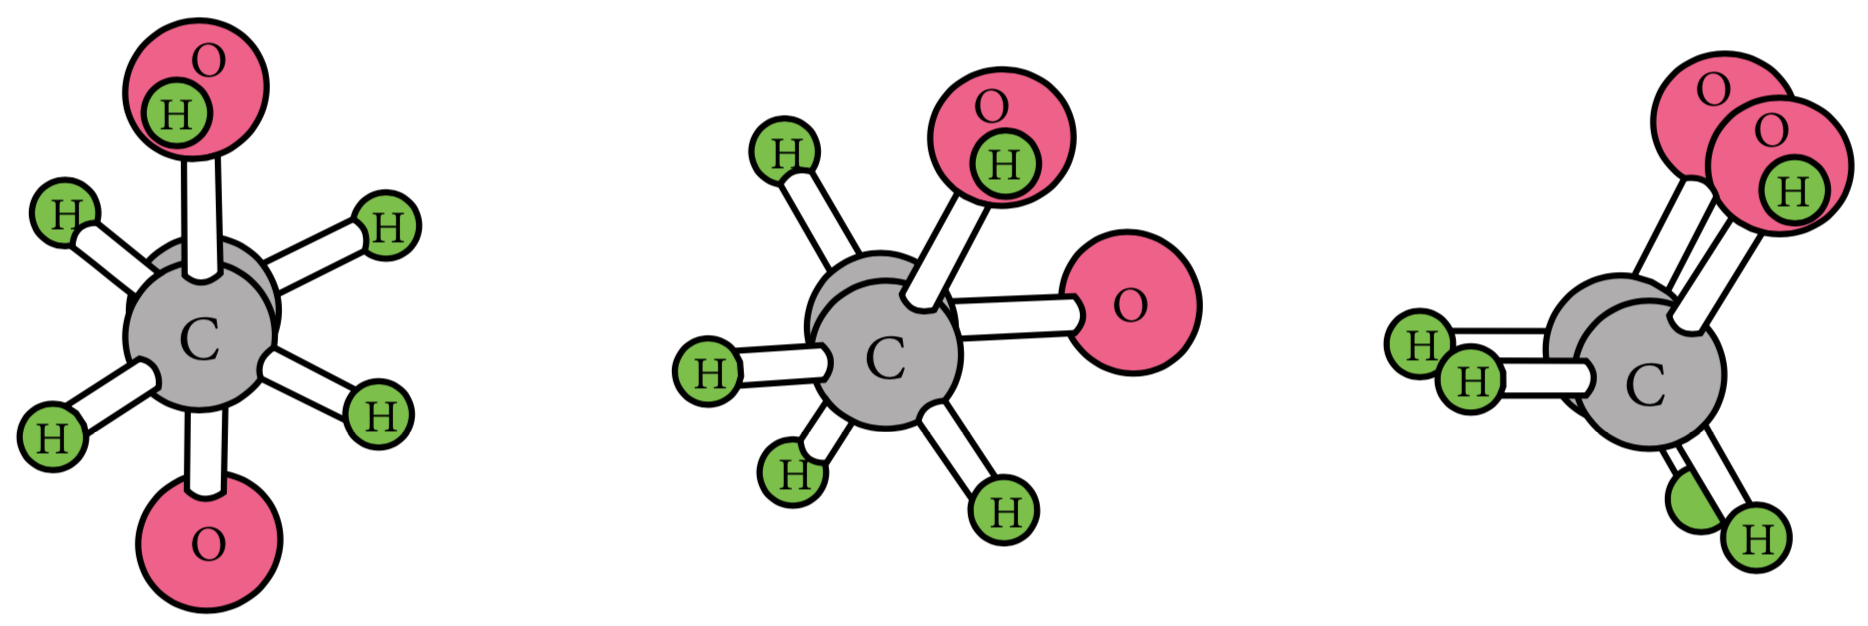
\includegraphics[width=0.9\textwidth]{coformers-1.png}

\caption{\small{Simple example of three coformers of ethylene glycol \cite{creighton2010biophysical}.}}

\label{fig:generation-of-microcan_state}
\end{minipage} 
\end{figure}

%Any conformation of a molecule of known covalent structure can be specified by the rotations about its single bonds, generally measured by either the torsion angle or the dihedral angle. In general, interactions between neighboring atoms, usually steric repulsions, mean that not all bond rotations have the same free energy and are equally probable
%\begin{figure}[h]
%\centering
%\begin{minipage}[t]{0.9\textwidth}
%\centering
%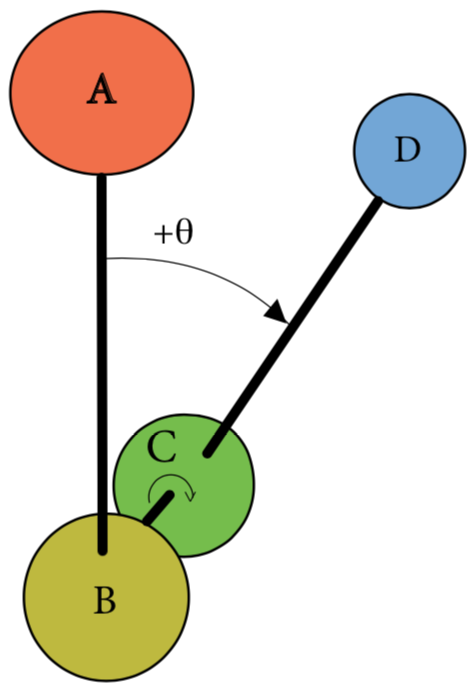
\includegraphics[width=0.22\textwidth]{./images/dihedral-0.png}
%\hspace{1cm}
%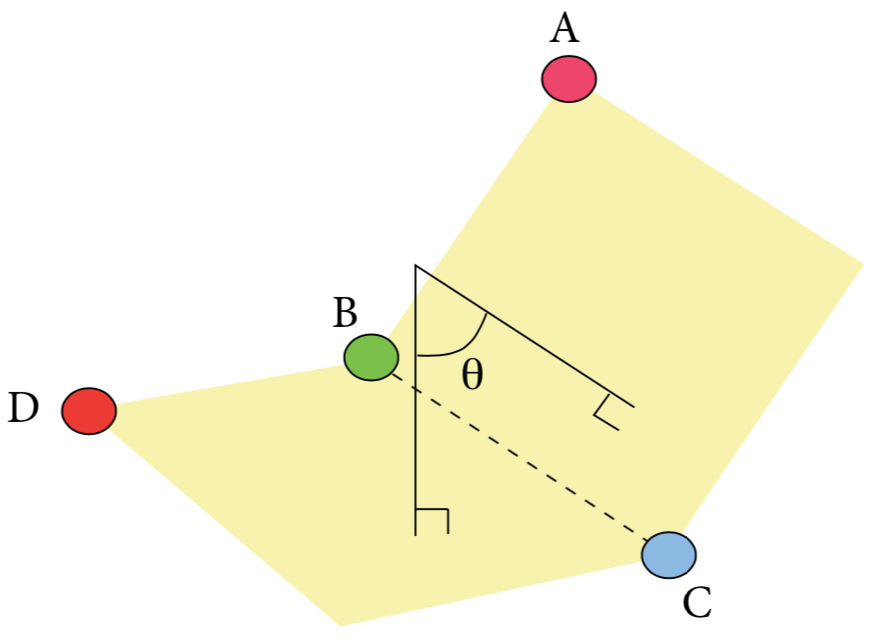
\includegraphics[width=0.45\textwidth]{./images/improper.png}
%
%\caption{\small{On the left: the torsion angles within a molecule that refer to the rotations about individual covalent bonds linking a pair of atoms; they are defined using two further atoms bonded to the first pair of atoms.  \cite{creighton2010biophysical}.}}
%
%\label{fig:generation-of-microcan_state}
%\end{minipage} 
%\end{figure}

A large biological macromolecule can have a stable, fixed 3-D structure, referred to as its native conformation, if it has sufficient stabilizing interactions between its various atoms. Although most of the conformation is fixed and it is considered a single conformation, parts of the molecule may still be flexible and able to undergo rotations about certain bonds. The average overall conformation can be considered a macro-conformation, whereas the variations resulting from flexibility define various micro-conformations. Interconverting different macro-conformations requires a cooperative change of a number of bond rotations simultaneously, whereas micro-conformations are interconverted by changes of just one or a few bond rotations. These cooperative changes will usually occur only slowly or infrequently under physiological conditions, although it can be speeded up dramatically under denaturing conditions. This relatively slow interconversion of the two macro-conformations is described as a conformational change, in which the macromolecule has been converted from one family of micro-conformations to an experimentally distinguishable family of other micro-conformations
\cite{creighton2010biophysical}.

In the case of a protein, its conformations will depend whether on the structures and conformational properties of their residues that on the environment -- especially the relative interactions of the protein with the solvent and with itself.

In this picture, the conformational entropy is a measure of the ability to adopt a number of such conformations that stabilizes the flexible state. A single conformation will be adopted only if the interactions stabilizing that particular conformation are sufficiently strong to overcome the conformational entropy tending to keep the protein unfolded. The number of micro-conformations and the conformational entropies of proteins can be very large. For example, if each residue can adopt an average of $j$ conformations, and there are $N$ residues in the protein, the total number of conformations possible will be approximately $j^N$. If the reasonable assumption is made that $j$ is $8$ and $N$ is $500$, there will be $8^{500}$ ($\approx 10^{452}$) conformations possible, a truly astronomical number. Of course, some of these conformations will not be feasible because they would have atoms of the protein overlapping in space, the excluded volume effect. There is still, however, much scope to be conservative and predict an astronomical number of conformations. For example, even a short protein of 100 residues in which each residue could adopt only two different conformations could adopt more than $10^{30}$ different protein conformations. If all these conformations have similar free energies, each would have only a very small probability of occurring in a molecule. At 25 %\textdegree 
$^\circ$ C, the free energy contribution of the conformational entropy for a protein in which each residue can adopt 10 conformations will be 1.36 $N$ kcal/mol. Consequently, for any one conformation to predominate will require, on average, stabilizing interactions $>$1.36 kcal/mol/residue. In the absence of such stabilizing interactions, a protein will tend to exist in many different conformations. However, proteins and nucleic acids are able to adopt single folded conformations that predominate. Such stable conformations can be considered macro-conformations, in contrast to the micro-conformations that are adopted only transiently \cite{creighton2010biophysical}.


In the last years, there is a growing interest in the protein configurational entropy as a major factor in controlling the protein activities associated with signaling, regulation, and recognition.

a field of a growing interest is the protein configurational entropy as a major factor in controlling the protein activities associated with signaling, regulation, and recognition.
In this context, \\
- copiare un po' dall'articolo koreano e da quello vecchio

\newpage

In this regard, it was a keen insight to suppose that the protein configurational entropy ($S_\text{config}$) may be characterized just by two terms, i.e., the conformational ($S_\text{conf}$) and vibrational ($S_\text{vib}$) components.
The conformational component is associated with the number of accessible free-energy wells, whereas the vibrational component reflects the average width of the individual wells. (Although they are often used interchangeably, we shall refer to ``conformational'' entropy as a subcategory of ``configurational'' entropy as just described.) -> questo perché nel processo di folding e unfolding $S_\text{vib} \simeq 0$ e quindi $S_\text{config} = S_\text{conf} + S_\text{vib} \simeq S_\text{conf}$

Dissecting $S_\text{config}$ into $S_\text{conf}$ and $S_\text{vib}$ enables one to characterize modulations of the free-energy landscape caused by intrinsic and extrinsic factors in simple terms; furthermore, it will facilitate the discovery of molecular mechanisms underlying protein activities (in particular, those of intrinsically disordered proteins).

Configurational entropy, however, is known as one of the most difficult thermodynamic quantities to estimate, and a significant amount of effort has been devoted to developing computational methods for dealing with this quantity. 

Here, we propose a computational approach from a different perspective that is based on the classification of protein
dynamics on the free-energy landscape into conformational and vibrational contributions (Figure 1). 


\cite{karplus1987configurational}

The aim of this thesis is to study 
\newpage

In this context, studying the association processes that bring to the formation of the binding between a protein and its ligand, it is possible to decompose the free energy of the association of the two molecules into a summation of favorable and unfavorable contributions. The mainly unfavorable contribution is due to the loss of the three translational and three rotational degrees of freedom that lead to a considerable decrease of the entropy of the system. Generally, it is assumed that this contribution is offset by favorable enthalpy of binding and entropic contributions, such as the hydrophobic effect, changes in the protonation state and solvent or counterion release. Nevertheless, there is another mechanism by which a significant amount of entropy can be recovered, namely, due to the creation of some new internal degrees of freedom in the complex \cite{tidor1994contribution}.

Indeed, because electrostatic interactions and hydrophobic bonds are not rigid or specific and the association is an outcome of such noncovalent interactions, the associating units (i.e. the protein and the ligand) have a considerable freedom of relative motion. This freedom, corresponding to an increase in flexibility for the complex and manifested by changes in its vibrational spectrum, is able to lead to a significant positive contribution for the entropy of the association (aside from the contribution from solvent effects, such as the hydrophobic effect) \cite{steinberg1963entropy}.

During the years, theoretical normal mode analyses, used to estimate this vibrational changes, have suggested that this effect is likely to be thermodynamically important and, in 2004, a first experimental determination of the vibrational changes has been achieved by Balog et al. Using inelastic neutron scattering, they showed that the vibrations of the complex soften significantly at low frequency (less then 2.5 meV) relative to the unbound protein. Deriving the resulting free-energy change from the variation in the density of states, they found that this effect contributes significantly to the binding equilibrium \cite{balog2004direct}.

Anyway, there remains much to learn about the various contributions to ligand binding free energies. Indeed, whether the vibrational softening effect seen here is general for protein-ligand interactions remains to be determined. The direct access to the vibrational density of states provided by inelastic neutron scattering holds promise for the study of vibrational thermodynamic changes in many biomolecular association processes \cite{balog2004direct}. 

Hence, to better understand this phenomena, in 2011 Balog et al., using computer simulations, recreated the system studied in the 2004 and reproduced the experimental results with an atomic detail normal-mode analysis to perform a characterization of the observed vibrational change.
With these simulations they obtain several interesting results concerning the nature of the vibrational changes in the specific protein-ligand complex studied\footnote{Some of these results concern the identification of the residues most affected by ligand binding and their contribution to protein compressibility \cite{balog2011vibrational}.}. However, as they report in their paper, these results cannot be generalized to other proteins and ligands since the effect depends on the strength of the interactions involved. 

Furthermore, the present analysis concentrates on the harmonic component of the dynamics.

oreover, they did not explain in detail the effect that the changes in the vibrational modes of the complex have in the vibrational spectrum of the hydration water.


%\section{Experimental evidence - A brief overview of the neutron scattering results}
